\chapter{Theoretical Foundations}\label{chapter_Theoretical_Foundations}
% Theoretical Foundations

% UTS Clustering Pattern Recognition Techniques – DTW-based.
% Spatio-Temporal Modeling
% Uni-Variate Time Series Data Mining: Clustering and Classification
% Uni-Variate Time Series Analysis: Forecast Models 

% Spatio-Temporal Predictive Queries – From DB to PSS     
% Discussion  

% Introduction ST Domain and Data
In this work, we are interested in processes from Spatio--Temporal domains with high volumes of data. 
%The analysis of this kind of data is still challenging and time consuming. The real-world processes in these domains are spatio-temporal in nature, a number of data collection methodologies have been devised to record the spatial and temporal information of every measurement in the data, referred to as spatio-temporal data.
%ST Data Discussion
A quality of spatio--temporal data that distinguish it from other data is the presence of dependencies among measurements induced by the spatial and temporal dimensions. The data instances are structurally related to each other in the context of space and time and show varying properties in different spatial regions and time periods \cite{Atluri2018}. 

% ST Data Properties
Thus, space and time introduce a variety of spatio--temporal data types and representations. They have two generic properties: (i) auto-correlation, meaning that observations made at nearby locations and time stamps are not independent but are correlated with each other, and (ii) heterogeneity, (or non-stationarity) both in space and time in varying ways and levels. These properties imply that spatial observations have consistent values at nearby locations, and show a smooth variation in temporal observations; as for the heterogeneity in space and time, it requires the learning of different models for varying spatio-temporal regions \cite{Wikle2019}

% Introduction and Focus to Time Series -- Univariate
In particular, we are interested in spatio--temporal data with the representation that involves treating spatial locations as objects and using the measurements collected from a spatial location over time to define the features. This type of data are time-series and in particular we are interested in univariate time-series:

% Time Series definition
\begin{definition}[Time Series]
	An ordered sequence of values of a variable at equally spaced time intervals. 
\end{definition}

\begin{definition}
	Univariate time-series, a univariate time series is the simplest form of temporal data and is a sequence of real numbers collected regularly in time, where each number represents a values.
\end{definition}

Several applications represented by this type of data exist, and depending of the solution proposed for the problem studied, it is necessary to use specific techniques and methods. We are interested in those to identify groups of time series that show similar temporal activity and are located nearby in space, recognize some temporal patterns that commonly repeat in a number of time series. At the same time, we are interested in techniques that use time series as input features to predict a target variable, in order to generate models that can predict the value of a time series at a future time stamp using its historical values.

%% Round-up intro
%In applications, such as climate science, one of the goals is to group locations that experience similar climatic phenomenon over time. In this case, locations are treated as instances/objects and features are defined based on climate variables measured over time \cite{Atluri2018}.
%
%%Examples of time series data include gross domestic product, sales volumes, stock prices, weather attributes when recorded over a time spread of several years, months, days, hours, and so on. The frequency of observation depends on the nature of the variable and its applications. For example, information about weather attributes could be available at every day or hourly. In other applications we can consider several physical processes which generate time series data at fraction of a second (Ex. Electrocardiogram readings(ECG)). 
%
%% Time Series Pattern Recognition and Clustering, and Classification
%Several fields of research have been studied in considerable detail by both database and pattern recognition communities for different domains of time series data \cite{KeoghKasetty2002}. In the context of time series data mining, one problem is how to represent the time series data. Based on the time series representation, it is possible to consider different mining tasks and we focus into the following fields: pattern discovery and clustering, and classification. 
%
% Chapter Outline
In Section \ref{Sec:TimeSeriesClustering} and \ref{Sec:TimeSeriesClassification} we introduce methods and techniques to find groups of time-series with high similarity and \ref{Sec:TimeSeriesForecast}

\section{Clustering}
\label{Sec:TimeSeriesClustering}

% Clustering definition and applications
Clustering is a data mining technique where similar data are placed into related or homogeneous groups without advanced knowledge of the groups' definitions. In detail, clusters are formed by grouping objects that have maximum similarity with other objects within the group, and minimum similarity with objects in other groups. It is a useful approach for exploratory data analysis as it identifies structure(s) in an unlabelled dataset by objectively organizing data into similar groups. According to \cite{Aghabozorgi2015}, time series clustering can be defined as follows:

\begin{definition} Time-series clustering, given a dataset of $n$ time-series data $\mathcal{D} = \{ \mathcal{S}_1, \mathcal{S}_2, \ldots, \mathcal{S}_n\}$; the process of unsupervised partitioning of $\mathcal{D}$ into $\mathcal{C} = \{C_1, C_2, \ldots C_k\}$, in such a way
that homogenous time-series are grouped together based on a certain similarity measure, is called time-series clustering. Then, $C_i$ is called a cluster, where $\mathcal{D} = \bigcup_{i=1}^{k} C_{i}$ and $C_i \cap C_j \neq \emptyset$ for $i \neq j$.
\end{definition}

% Similarity Measure
%http://practicalquant.blogspot.com/2012/10/mining-time-series-with-trillions-of.html
We need to consider a similarity measure to calculate the similarity among the whole time-series. This is not a simple process, time-series data are naturally noisy and include outliers and shifts, in some cases the length of time-series varies and the distance among them needs to be calculated \cite{Pal2017}. In the literature we found several approaches to find similar time-series and we are interested in a shape--based approach, shapes of two time-series are matched as well as possible, by a non-linear stretching and contracting of the time axes (considering raw time-series data).

\subsection{Shape-based Distance Algorithms}
\label{sec:ShapeBasedDistance}

Shape-based distance algorithms usually employ conventional clustering methods, which are compatible with static data while their distance/similarity measure has been modified with an appropriate one for time-series. A commonly used shape--based similarity measure is the Dynamic Time Warping (DTW) \cite{Sakoe1978} and its variants. DTW is a generalization of classical algorithms for comparing discrete sequences to sequences of continuous values, and leverages dynamic programming to calculate an optimal match between two sequences of feature vectors by allowing for stretching and compression of sections of the sequences. 
%For univariate time--series data, several clustering techniques exist (See Section \ref{Sec:TimeSeriesClustering}). Since we are interested in leveraging the temporal behavior of the spatio--temporal domain, we adopt a shape--based similarity measure, i.e. we analyze the similarity of time--series based on the evolution of its shape over time. The similarity metric known as Dynamic Time Warping (DTW) \cite{Sakoe1978} is based on dynamic programming, it calculates an optimal match between two sequences of feature vectors by allowing for stretching and compression of sections of the sequences. 


%The time of occurrence of patterns is not important to find similar time-series in shape. As a result, elastic methods [108,113] such as Dynamic time Warping (DTW) [114] is used for dissimilarity calculation. Using this definition, clusters of time-series with similar patterns of change are constructed regardless of time points, for example, to cluster share price related to different companies which have a common pattern in their stock independent on its occurrence in time-series [112]. Similarity in time is an especial case of similarity in shape. A research has revealed that similarity in shape is superior to metrics based on similarity in time [115].
%http://practicalquant.blogspot.com/2012/10/mining-time-series-with-trillions-of.html

%Dynamic time warping (DTW) is a generalization of classical algorithms for comparing discrete sequences to sequences of continuous values, introduced in \cite{Sakoe1978}.

Given two time series, $\mathcal{S}_{1} =\{s_{11}, s_{12}, \ldots, s_{1n}\}$ and $\mathcal{S}_{2} = \{s_{21}, s_{22}, \ldots, s_{2m}\}$, DTW aligns the two series so that their difference is minimized. To this end, an $n \times m$ matrix where the $(i, j)$ element of the matrix contains the distance $d(s_{1i}, s_{2j})$ between two points $s_{1i}$, and $s_{2j}$ . The Euclidean distance is normally used. 

A warping path, $W = w_{1} , w_{2}, \ldots w_{k}, \ldots, w_{K}$ where $\max(m, n) \leq K \leq m + n-1$, is a set of matrix elements that satisfies three constraints: boundary condition, continuity, and monotonicity. 

The boundary condition constraint requires the warping path to start and finish in diagonally opposite corner cells of the matrix. That is $w_{1} = (1, 1)$ and $w_{K} = (m, n)$. The continuity constraint restricts the allowable steps to adjacent cells. The monotonicity constraint forces the points in the warping path to be monotonically spaced in time. The warping path that has the minimum distance between the two series is of interest. Mathematically, 
\begin{equation}
d_{DTW} = \min \frac{\sum_{k=1}^{K} w_{k}}{K}
\end{equation}

Dynamic programming can be used to effectively find this path by evaluating the following recurrence, which defines the cumulative distance as the sum of the distance of the current element and the minimum of the cumulative distances of the adjacent elements:

\begin{equation}
d_{cum}(i,j) = d(s_{1i}, s_2{j}) + \min{d_{cum} (i-1, j-1), d_{cum} (i-1, j ), d_{cum} (i, j-1)}.
\end{equation}

\subsection{$k$--Medoids Clustering }

% Clustering representative or prototype description
% TODO [150] y [151]
Another aspect to consider in time-series clustering the most common way to approach optimal Steiner sequence is to use cluster medoid as the prototype or representative [150]. In this approach, the centre of a cluster is defined as a sequence which minimizes the sum of squared distances to other objects within the cluster. Given time-series in a cluster, the distance of all time-series pairs within the cluster is calculated using a distance measure such as Euclidean or DTW. Then, one of the time-series in the cluster, which has lower sum of square error is defined as medoid of the cluster [151]. Moreover, if the distance is a non-elastic approach such as Euclidean, or if the centroid of the cluster can be calculated, it can be said that medoid is the nearest time-series to centroid.

% K--Medoid
A partitioning clustering method makes $k$ groups from $n$ unlabelled objects in the way that each group contains at least one object. One of the most used algorithms of partitioning clustering is $k$-Means, where each cluster has a representative which is the mean value of its objects. The main idea behind $k$-Means clustering is the minimization of the total distance (typically Euclidian distance) between all objects in a cluster from their cluster center (representative).

Another member of partitioning family is $k$-Medoids (PAM) algorithm \cite{Kaufman2009}, where the representative of each cluster is one of the nearest objects to the centre of the cluster. In $k$-Medoids clustering algorithm, the number of clusters $k$, has to be pre-assigned, which is not available or feasible to be determined for many applications, so it is impractical in obtaining natural clustering results and is known as one of their drawbacks in static objects [21] and also time-series data [15]. It is even worse in time-series because the datasets are very large and diagnostic checks for determining the number of clusters is not easy. %Accordingly, authors in [171] investigate the role of choosing correct initial clusters in quality and time-execution of $k$-Means in time-series clustering.  
$k$-Means and $k$-Medoids algorithms make clusters which are constructed in a `crispy' manner and it means that an object is either a member of a cluster or not. They use raw univariate time-series of equal length. 

% Methods and techniques to find the optimal number of $k$


% Elbow

% Sihouette Index or Score


In the next Section we describe some theoretical aspects for time-series classification, another 

\section{Time Series Classification} 
\label{Sec:TimeSeriesClassification}

In general, classification consists of predicting the correct class of a given data point using a labeled training set. In the case of Time Series Classification, we consider the data points as the whole time series, and the task consists of predicting its correct label. Similar to unsupervised learning, traditional classification approaches can provide a basic baseline for solving this underlying time-series classification task. However over the past two decades, research has shown that designing algorithms that can exploit the temporal information is a need in order to achieve high classification accuracy \cite{Fawaz2019}. 

\begin{definition}
A dataset $D=\{(\mathcal{S}_1,Y_1),(\mathcal{S}_2,Y_2), \ldots ,(\mathcal{S}_N,Y_N)\}$ is a collection of pairs $(\mathcal{S}_i,Y_i)$ where $\mathcal{S}_i$ is univariate time series with $Y_i$ as its corresponding one-hot label vector.  For a dataset containing $k$ classes, the one-hot label vector $Y_i$ is a vector of length $k$ where each element $j \in [1,k]$ is equal to 1 if the class of $X_i$ is $j$ and $0$ otherwise.
\end{definition}

% Traditional Methods for Time Series Classification
Using a classification method we will be able to learn from data about the membership relation between elements of the domain and representatives, and then use this learning to classify new time-series. 

% Use of Neural Networks for TS Classification

% Deep Learning for TS Classification

% CNN for Time Series
Convolutional Neural Networks (CNNs) come under the umbrella of Deep Learning, a subset of machine learning that uses multi-layered artificial neural networks to deliver state-of-the-art accuracy in tasks such as object detection, speech recognition, language translation and others \cite{}. Typically, a CNN maps 2D input (images) either to categorical outputs (in case of classification problems) or to a real value (in case of regression based problems). We describe the use of 1D CNNs for time-series data. Typically, a CNN model involves two kinds of layers: Convolution and Multilayer Feed Forward. 

Convolution layer, involves the convolution operation that is performed as a window of weights slides across an image, where an output pixel produced at each position is a weighted sum of the input pixels covered by the window. The weights that parameterize the window remain the same throughout the scanning process. Therefore, convolutional layers can capture the shift-invariance of visual patterns and learn robust features.

Multilayer Feed Forward or fully connected layer is a structure where neurons from a layer is connected to all the neurons in the next layer, for a multiclass classification the dense layer is commonly used. Considering the \texttt{softmax} function onto the last layer, it creates a probability distribution over $K$ classes, and produces an output vector of length $K$. Each element of the vector is the probability that the input belongs to the corresponding class. The most likely class is chosen by selecting the index of that vector having the highest probability.

%The model uses the efficient Adam version of stochastic gradient descent and optimizes the mean sequared error loss function.
Once the model is defined, it can be fit on the training data and the fit model can be used to make a prediction. A CNN is typically composed of multiple alternating convolutional and pooling layers, followed by one or several fully connected layers. CNNs exploit local correlations by enforcing a local connectivity pattern between neurons of adjacent layers, namely, the inputs of neurons in the current layer come from a subset of neurons in the previous layer. This hierarchical architecture allows convolutional neural networks to extract more and more abstract representations from the lower layer to the higher layer. 


\section{Time Series Analysis and Forecast}
\label{Sec:TimeSeriesForecast}

% Spatio-Temporal Modeling
The basic objective of predictive learning methods is to learn a mapping from the input features (also called as independent variables) to the output variables (also called as dependent variables) using a representative training set. In spatio-temporal applications, both the input and output variables can belong to different types of ST data instances, thus resulting in a variety of predictive learning problem formulations. In the following, we discuss some of the predictive learning problems that are commonly encountered in ST applications based on the type of ST data instance used as input variables

% TS and UTS Data Recap to Introduce TSA
On the other hand, a successful utilization of time series data would lead to monitoring the evolution of a phenomenon over time. The field of time series analysis aims to utilize such data for several purposes that can be categorized as: to understand and interpret the underlying forces that produce the observed state of a system or process over time; to forecast the future state of the system or process in terms of observable characteristics.

% TS Data Characteristics for modeling
The nature of time series data includes: large in data size, high dimensionality and update continuously. Moreover time series data, which is characterized by its numerical and continuous nature, is always considered as a whole instead of individual numerical field \cite{Pal2017}. The 

\begin{itemize}
	\item Trend: A trend exists when there is a long-term increase or decrease in the data. It does not have to be linear. Sometimes we will refer to a trend as ``changing direction'', when it might go from an increasing trend to a decreasing trend.
	\item Seasonal A seasonal pattern occurs when a time series is a effected by seasonal factors such as the time of the year or the day of the week. Seasonality is always of a fixed and known frequency. 
	\item Cyclic A cycle occurs when the data exhibit rises and falls that are not of a frequency.
\end{itemize}

% Introduction TSA
One objective of time series analysis is to develop models that provide plausible descriptions for time series data. For this we consider the fact that time series data are usually not independent and the analysis must take into account the time order of the observations. As a consequence, when successive observations (time series) are dependent, future values may be predicted from past observations \cite{Mills2019}. Many applications are represented by stochastic time series, meaning that the future is partly determined by past values. Thus the exact predictions are impossible to determine and must be replaced by the idea that future values have a probability distribution, which is conditioned on a knowledge of past values. 

There are several possible objectives in analyzing a time series, in this Section we describe methods and techniques for prediction or forecast. %They rely on the idea that historical data include intrinsic patterns which carry useful information for the future description of the phenomenon investigated. These patterns are usually non-trivial to identify, and their discovery is one of the primary goals of the time series processing: the circumstances the patterns found will repeat and what types of changes they may suffer over time \cite{}. 
%
%In \cite{}, 
%\begin{definition}
%	A time series model for the observed data $\{s_{t}\}$ is a specification of the joint distributions (or possibly only the means and covariances) of a sequence of random variables $\{S_{t}\}$ of which $\{s_{t}\}$ is postulated to be a realization.
%\end{definition}
% TS- Forecast
In particular, time-series forecasting is a form of quantitative forecasting, it can be applied when three conditions exist: (1) Information about the past is available, (2) this information can be quantified in the form of numerical data, and (3) it can be assumed that some aspects of the past pattern will continue into the future. This last condition is known as the ``assumption of continuity'' \cite{Makridakis2008}; it is an underlying premise of all quantitative and many qualitative forecasting methods. Time series forecasting treats the system as a black box and makes no attempt to discover the factors affecting its behavior. Therefore, prediction of the future is based on past values of a variable and/or past errors, but not on explanatory variables which may affect the system. The objective of such time series forecasting methods is to discover the pattern in the historical data series and extrapolate that pattern into the future. 

% Types of Time Series Analysys

% Justification for Box-Jenkins Methods

% ARIMA and kNN for time series forecast
In this work we consider Auto Regressive Integrated Moving Average (ARIMA) as the time--series forecast method to generate predictive models. Also known as the Box-Jenkins model \cite{Chatfield2019}, ARIMA are the most general class of models for forecasting a time series which can be made to be ``stationary'' by differencing (when necessary). A random variable, that is a time series, is stationary if its statistical properties (mean and covariance) are all constant over time.  A stationary series has no trend, its variations around its mean have a constant amplitude, and its autocorrelations (correlations with its own prior deviations from the mean) remain constant over time.  A random variable of this form can be viewed (as usual) as a combination of signal and noise, and the signal (if one is apparent) could be a pattern of fast or slow mean reversion, or sinusoidal oscillation, or rapid alternation in sign, and it could also have a seasonal component. An ARIMA model can be viewed as a ``filter'' that tries to separate the signal from the noise, and the signal is then extrapolated into the future to obtain forecasts.

The ARIMA forecasting equation for a stationary time series is a linear (i.e., regression-type) equation in which the predictors consist of lags of the dependent variable and/or lags of the forecast errors.  The integrated components are useful when data has non-stationarity, and the integrated part of ARIMA helps in reducing the non-stationarity. The ARIMA applies differencing on time series one or more times to remove non-stationarity effect. The ARIMA$(p, d, q)$ represent the order for AR, MA, and differencing components. The $d$ component aims to detrend the signal to make it stationary and ARMA model can be applied to the de-trended dataset . 

% Time Series Forecast Error 
Accuracy measures, error statistics or measures, and loss functions are alternative ways of conveying information about the ability of a certain forecasting method to predict actual data, either when a model is fitted to such data, or for future periods (post-sample) whose values have not been used to develop the forecasting model \cite{Makridakis1993}. To measure the accuracy of forecast methods applied to univariate time series data, $s_{t}$ denote the observation at time $t$ and $\hat{s}_t$ denote the forecast of $s_{t}$.

We consider the following scale-dependent errors:
\begin{itemize}
	\item Mean Squared Error (MSE): Measures the average squared error of the predictions. For each point, it calculates square difference between the predictions and the target, and then average those values:
	\begin{equation}
	MSE = \frac{1}{n} \sum_{j=1}^{n} \left(s_j - \hat{s}_j\right)^{2}.
	\end{equation}
	
	The higher this value, the worse the model is. It is never negative, since we're squaring the individual prediction-wise errors before summing them, but would be zero for a perfect model .
	
	\item Root Mean Squared Error (RMSE): Represents the sample standard deviation of the differences between predicted and observed values (called residuals). Mathematically, it is calculated using this formula:
	\begin{equation}
	RMSE = \sqrt{\frac{1}{n} \sum_{j=1}^{n} \left(s_j - \hat{s}_j\right)^2}
	\end{equation}
	Often, the RMSE is preferred to the MSE as it is on the same scale as the data. Historically, the RMSE and MSE have been popular, largely because of their theoretical relevance in statistical modelling. However, they are more sensitive to outliers.
\end{itemize}

Also we consider percentage errors, they have the advantage of being unit-free, and so are frequently used to compare forecast performances between data sets. Measures based on percentage errors have the disadvantage of being infinite or undefined if $s_{j}=0$ for any $j$ in the period of interest, and having extreme values if any $s_{j}$ is close to zero. Another problem with percentage errors that is often overlooked is that they assume the unit of measurement has a meaningful zero \cite{Hyndman2006}. This observation led to the use of the so-called ``symmetric'' MAPE (sMAPE):

\begin{itemize}	
	\item Mean Absolute Percentage Error (MAPE):
	\begin{equation}
	MAPE = \frac{100}{n}\sum_{j=1}^{n} \frac{\left|s_j - \hat{s}_j\right|}{|s_j|}
	\end{equation}	
	\item Symmetric Mean Absolute Error (sMAPE):	
	\begin{equation}
	MAPE = \frac{200}{n}\sum_{j=1}^{n} \frac{\left|s_j - \hat{s}_j\right|}{\left(s_{j}+\hat{s}_{j}\right)}
	\end{equation}	
	
\end{itemize}

%It is defined by sMAPE=mean(200|yt−^yt|/(yt+^yt)).
%However, if yt is close to zero, ^yt is also likely to be close to zero. Thus, the measure still involves division by a number close to zero, making the calculation unstable. Also, the value of sMAPE can be negative, so it is not really a measure of “absolute percentage errors” at all.


\section{Problem Formalization}
\label{Sec:ProblemFormalization}

Let $\mathcal{D} = \{(\mathcal{S}, x, y): \,\, \mathcal{S} = \{s_{1}, s_{2}, \ldots, s_{t}\}$ is a univariate time--series, and $(x,y) \in \mathbb{R}^{2}\}$, represents a spatio-temporal domain. Denote by $\mathcal{G} = \{g: \mathbf{S} \to \mathbf{S}$ such that $g(\mathcal{S}) = \mathcal{S}\}$, the set of temporal predictive models for $\mathbf{S} \subseteq \mathcal{D}$. Each predictive model $g\in \mathcal{G}$ is denoted as follows:
\begin{equation}
\label{eq:ModelDefinition}
g = \langle \mathbf{S}, A, \mathbf{p}, E, \varSigma \rangle,
\end{equation}
where:
\begin{itemize}[noitemsep,nolistsep]	
	\item $\mathbf{S}$: input dataset included in the spatio--temporal domain $\mathcal{D}$,
	%		\item $I$: algorithm's input dataset size/shape (For DL Models),
	\item $A$: learner or hypothesis set,
	\item $\mathbf{p}$: model parameters (number of time-units to obtain the generalization error ($tp$), number of time-units to forecast ($tf$)),
	\item $E$: generalization error,
	\item $\varSigma$: implementation/execution quality metrics.
\end{itemize}

%TODO Extend the existence for several competing models.
\noindent In this context, given a predictive spatio--temporal query $Q$ denoted as:
\begin{equation} \label{eq:predictivequery}
Q = \langle R, t_{p}, t_{f}, Q_{m} \rangle,
\end{equation}
where:
\begin{itemize}[noitemsep,nolistsep]	
	\item $R$: represents the size/shape/type of interest region,
	\item $t_{p}$: $\{s_{t-t_p}, s_{t-t_{p}+1}\ldots, s_{t}\}$ number of steps used for  prediction,
	\item $t_{f}$: $\{s_{t+1}, \ldots, s_{t+t_f}\}$ number of steps to predict ($n\geq 1$),
	\item $Q_{m}$: represents users qualitative measurements to evaluate the predictive output.
	%\item $Y_{Q}$: prediction output.
\end{itemize}

We formally define our problem: Let the spatio--temporal domain characterization $\mathcal{D} = \bigcup_{i=1}^{n} \mathbf{S_i}$ and $\mathcal{G}$ the set of temporal models for a single element of $\mathbf{S_i}$ that accounts for the generalization error bounds for the elements in $\mathbf{S_i}$. Given $Q = \langle R, t_p, t_f, Q_{m} \rangle$:

\begin{equation}
\forall \mathcal{S} \in R: \exists g \in \mathcal{G'} \,\,\textrm{such that} \,\, \argminA_{g\in\mathcal{G'}} E_{g}(R).
\end{equation}

%TODO Change the argmin 
\noindent In Figure \ref{fig:time-series}, we show the elements involved in the formalization of our problem:
\begin{center}
	\begin{figure}[htb]
		%\begin{minipage}[b]{0.8\textwidth}
		\centering
		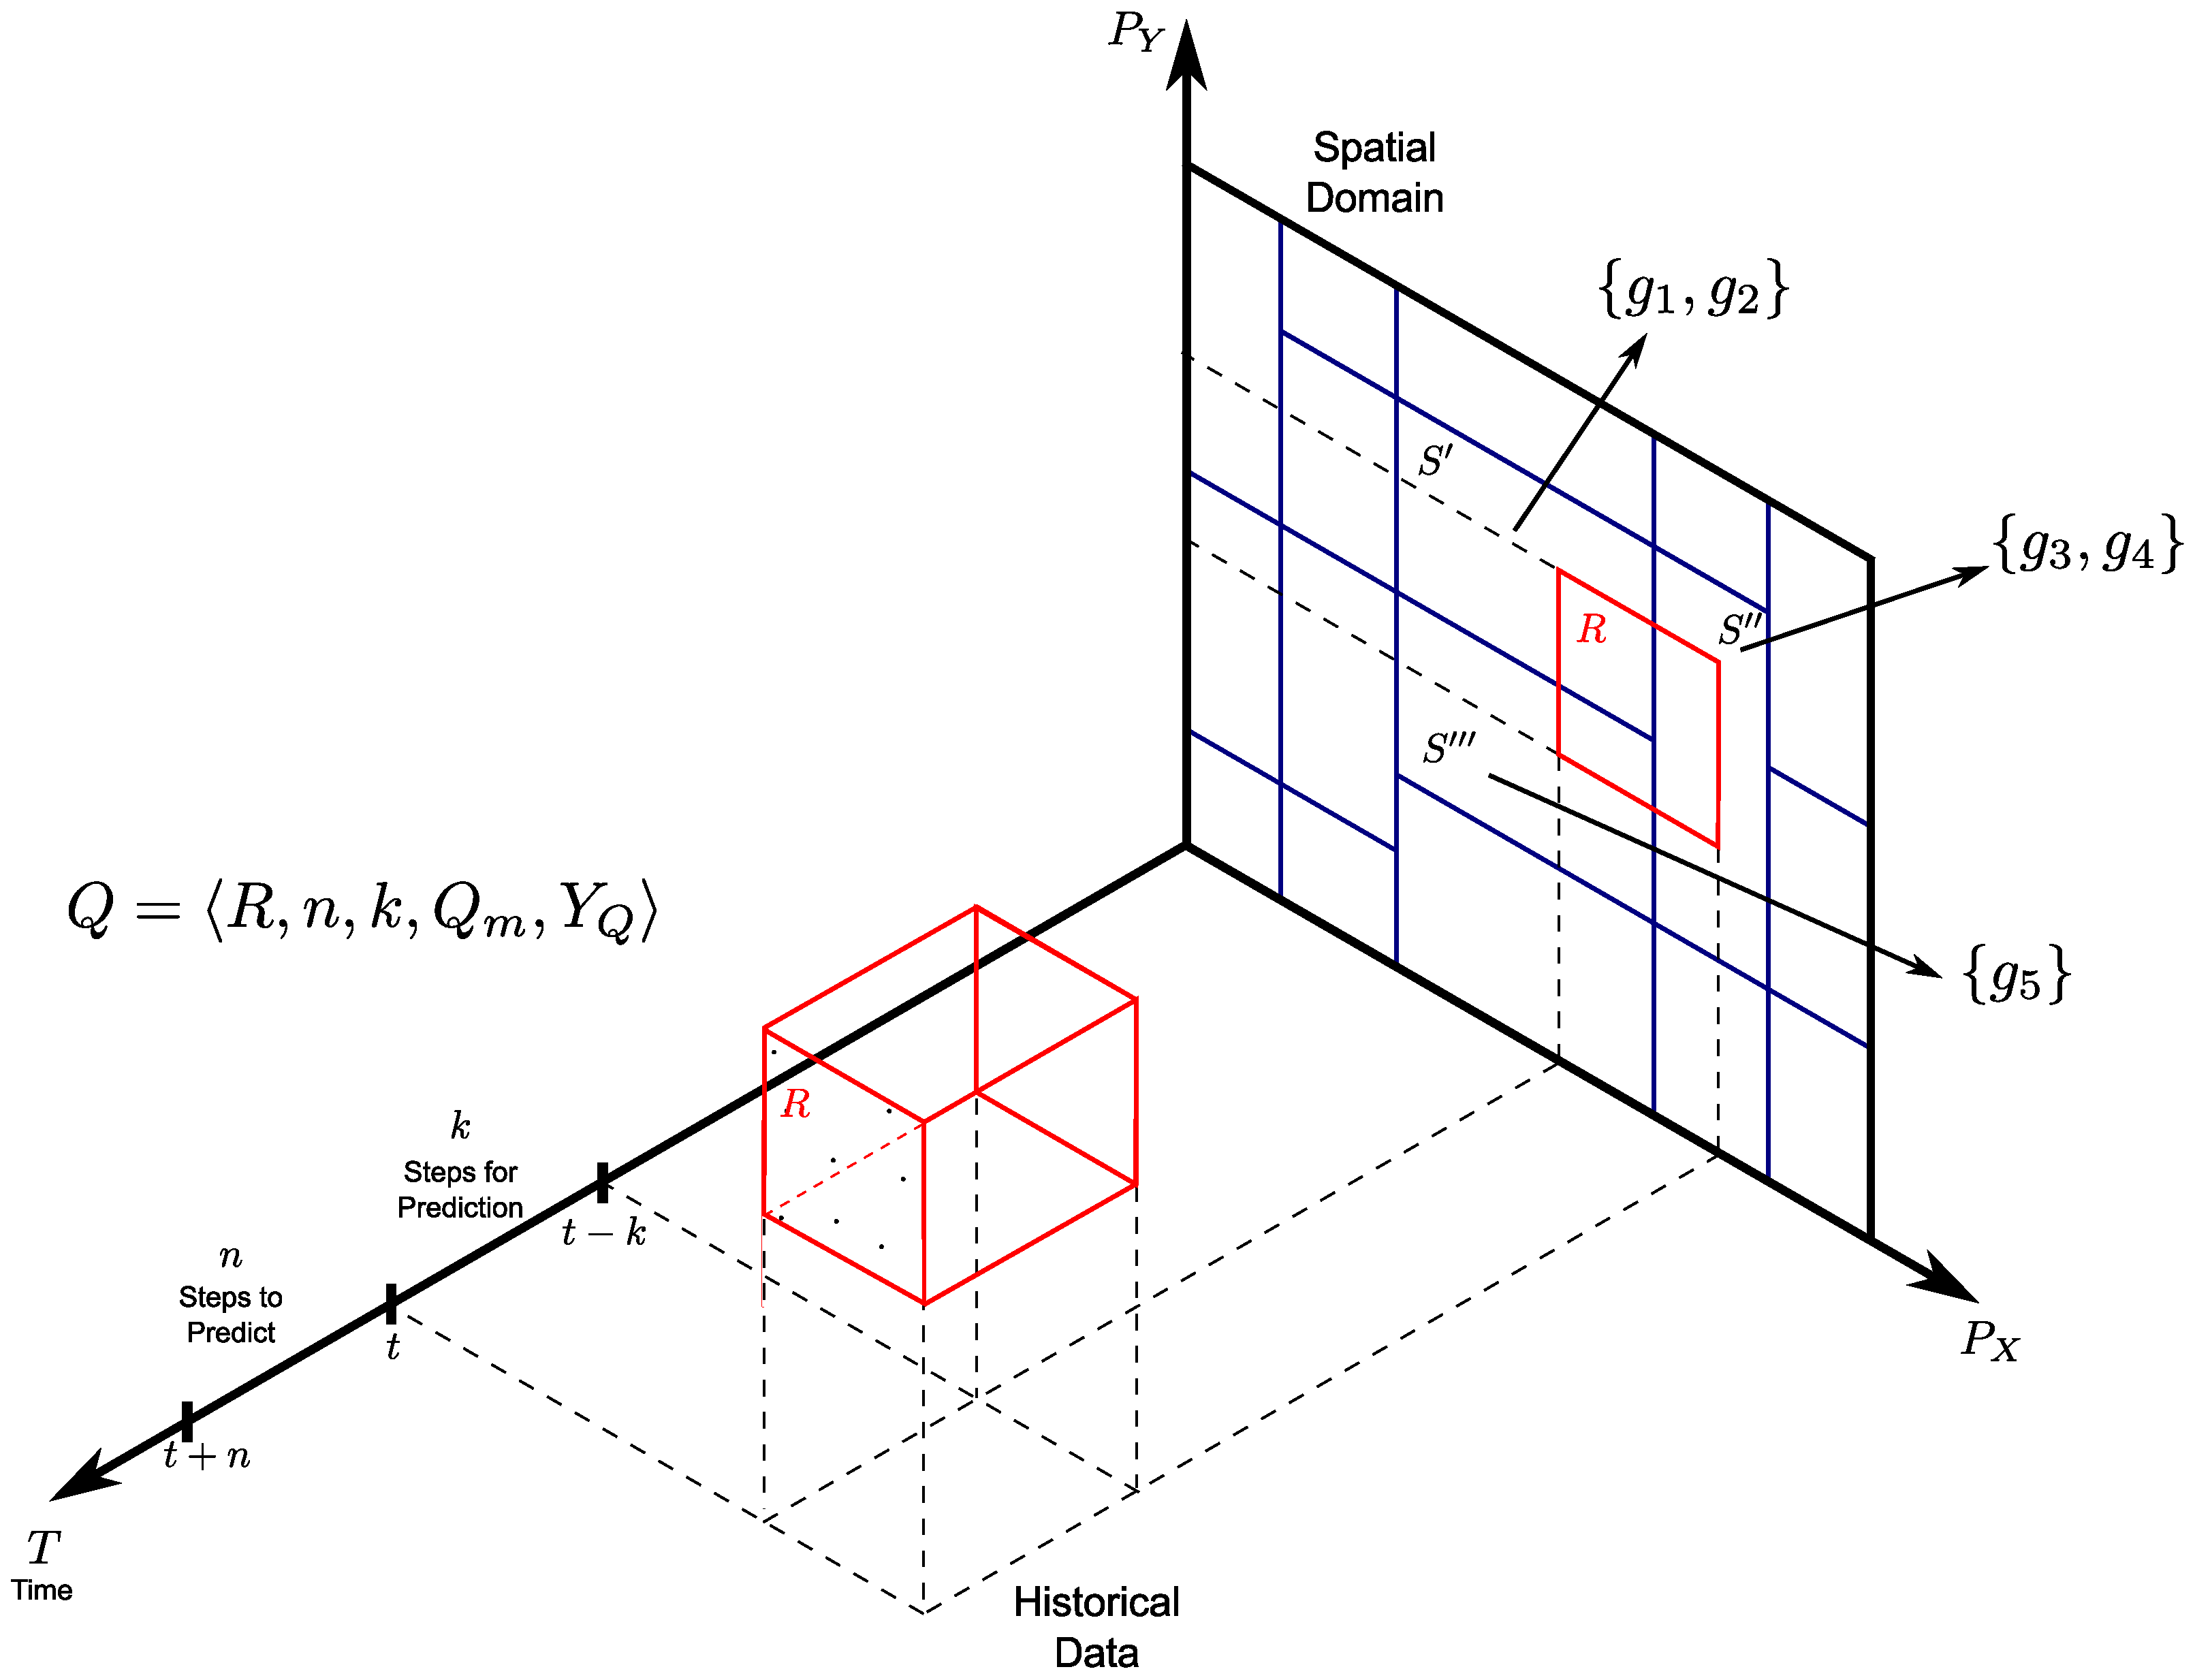
\includegraphics[scale=0.15]{../Figures/RepresentationTimeSeries}
		\caption{Predictive Spatio--Temporal Queries.}
		\label{fig:time-series}
		%\end{minipage}
	\end{figure}
\end{center}

\section{Final Considerations}